\chapterA{Modelado}
\section{Introducción}
La fase de modelado es la segunda etapa del proceso de Diseño Guiado por Objetivos (DGO). En esta fase, partiremos de la lista de factoides que
obtuvimos en la etapa anterior y con ella diseñar los prototipos de personas que serán los potenciales usuarios de la misma, representando además
las principales características que extrajimos de los factoides.

Para poder lograr este objetivo, tenemos que realizar una serie de pasos.
\section{Planificación del hito}
Para poder planificar este hito correctamente, hemos identificado en una Hoja de cálculo (ver figura \ref{fig:planif-hito2}) las distintas tareas que tenemos que 
realizar, junto al intervalo de fechas en el que se encuentra prevista su realización y el / los responsables de dicha tarea.
\begin{figure}[H]
    \centering 
    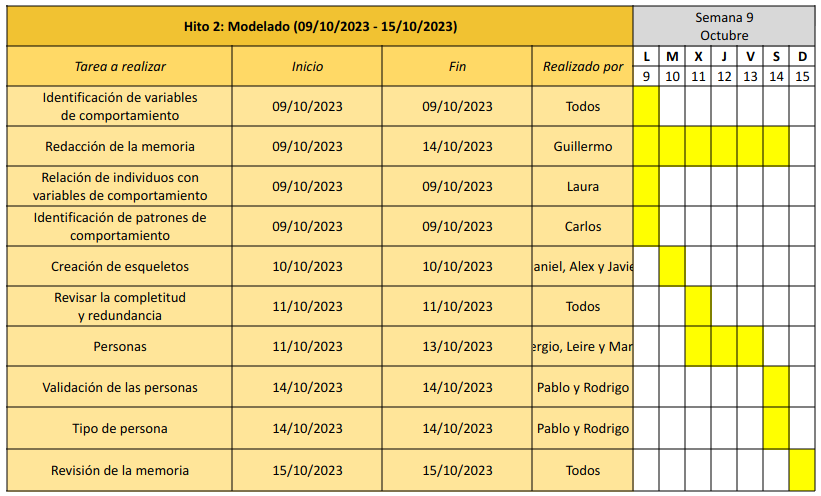
\includegraphics[width=0.8\textwidth]{./Imagenes/Planificaciones/Planif-hito2.png}
    \caption{Planificación Hito 2}
    \label{fig:planif-hito2}
\end{figure}

\section{Identificación de variables de comportamiento}
\section{Relación de individuos con variables de comportamiento}
\begin{table}[H]
    \centering
    \begin{tabular}{l|l|l|l|l|l|l|}
        \cline{2-5}
                                                                & Madi        & Sofía                          & Alberto            & Beatriz                         \\ \hline
        \multicolumn{1}{|l|}{Rango de edad}                     &             & 18 - 25                        & 18 - 25            & 18 - 25                         \\ \hline
        \multicolumn{1}{|l|}{Estado civil}                      & Si          & Soltera                        & En pareja          & En pareja                       \\ \hline
        \multicolumn{1}{|l|}{Organización de viajes}            & Si          & Si                             & Si                 & Si                              \\ \hline
        \multicolumn{1}{|l|}{Uso de comparadores de viajes}     & No          & \multirow{2}{*}{Kayak, Skyscanner, Trivago}     & No                 & \multirow{2}{*}{eDreams, comparador de Google}   \\ \hline
        \multicolumn{1}{|l|}{Frecuencia de viaje}               & Baja        & Media                          & Alta               & Baja                            \\ \hline
        \multicolumn{1}{|l|}{Tipo de viaje}                     & Trabajo     & Ocio                           & Ocio               & Ocio                            \\ \hline
        \multicolumn{1}{|l|}{Discapacidad}                      & No          & No                             & No                 & No                              \\ \hline
        \multicolumn{1}{|l|}{Acompañante}                       &             & Familia                        & Pareja             & Familia                         \\ \hline
        \multicolumn{1}{|l|}{Medio de transporte más frecuente} & Tren        & Transporte público             & Vehículo propio    & Vehículo propio                 \\ \hline
        \multicolumn{1}{|l|}{Uso de tecnología}                 &             & Alto                           & Alto               & Alto                            \\ \hline
        \multicolumn{1}{|l|}{Viaje nacional}                    & Si          & Si                             & Si                 & Si                              \\ \hline
        \multicolumn{1}{|l|}{Viaje internacional}               & Si          & Si                             &                    & Si                              \\ \hline
        \multicolumn{1}{|l|}{Trabaja}                           & Si          & No                             & Si                 & No                              \\ \hline
        \multicolumn{1}{|l|}{Gusto por viajar}                  &             & Si                             & Si                 & Si                              \\ \hline
        \multicolumn{1}{|l|}{Nivel de ahorro}                   & Alto        & Alto                           & Medio              & Alto                            \\ \hline
    \end{tabular}
    \caption{Tabla de relación de los individuos con las variables de comportamiento}
    \label{table:relacion-individuos-variables}
\end{table}

\section{Identificación de patrones de comportamiento}
Tras realizar el análisis de la matriz anterior hemos identificado los siguientes patrones de comportamiento:
\begin{itemize}
    \item La gente entre 18 y 25 años comparte un gusto por viajar y sobre todo viajes de ocio.
    \item La gente entre 18 y 25 años joven tiene un alto uso de la tecnología.
    \item Todos organizan viajes y casi todos tienen un nivel de ahorro alto. 
    \item La gente entre 18 y 25 años comparte el gusto por viajar.
    \item La mitad de las personas utilizan comparadores para organizar los viajes.
    \item La mitad de la gente entrevistada viaja con sus familiares.
    \item A casi todos los entrevistados les gustan los viajes internacionales.
    \item En general la frecuencia de viajes de los usuarios son media-bajas.
\end{itemize}

Vamos a tener dos tipos de personas. Personas que viajen por ocio, en general jóvenes, que se organicen sus propios viajes con un gusto por viajar. Y por otro lado tendremos otro tipo de personas que trabajen y que viajen por trabajo y estas personas no utilizan comparadores de viajes.

\section{Creación de esqueletos}
\section{Revisar la completitud y la redundancia}
\section{Personas}
\section{Validación de las personas}
\section{Tipos de personas}